\documentclass{beamer}
%
% Choose how your presentation looks.
%
% For more themes, color themes and font themes, see:
% http://deic.uab.es/~iblanes/beamer_gallery/index_by_theme.html
%
\mode<presentation>
{
  \usetheme{Madrid}      % or try Darmstadt, Madrid, Warsaw, ...
  \usecolortheme{beaver} % or try albatross, beaver, crane, ...
  \usefonttheme{serif}  % or try serif, structurebold, ...
  \setbeamertemplate{navigation symbols}{}
  \setbeamertemplate{caption}[numbered]
} 

\usepackage[english]{babel}

\usepackage[utf8x]{inputenc}
\usepackage{xcolor}
\usepackage{listings}
\usepackage{textpos}


\usepackage{verbatim}
\usepackage{filecontents}
\usepackage{siunitx}
\sisetup{per=slash, load=abbr}
\usepackage{tikz}
\usepackage{pgfplots}
\pgfplotsset{width=7cm,compat=newest}
\usepackage[autostyle=true,german=quotes]{csquotes}

% https://github.com/zemirco/tu-darmstadt-latex-thesis


% Farbpalette A
\definecolor{blau_1a}{RGB}{93,133,195}
\definecolor{blau_2a}{RGB}{0,156,218}
\definecolor{gruen_3a}{RGB}{80,182,149}
\definecolor{gruen_4a}{RGB}{175,204,80}
\definecolor{gruen_5a}{RGB}{221,223,72}
\definecolor{orange_6a}{RGB}{255,224,92}
\definecolor{orange_7a}{RGB}{248,186,60}
\definecolor{rot_8a}{RGB}{238,122,52}
\definecolor{rot_9a}{RGB}{233,80,62}
\definecolor{lila_10a}{RGB}{201,48,142}
\definecolor{lila_11a}{RGB}{128,69,151}

% Farbpalette B
\definecolor{blau_1b}{RGB}{0,90,169}
\definecolor{blau_2b}{RGB}{0,131,204}
\definecolor{gruen_3b}{RGB}{0,157,129}
\definecolor{gruen_4b}{RGB}{153,192,0}
\definecolor{gruen_5b}{RGB}{201,212,0}
\definecolor{orange_6b}{RGB}{253,202,0}
\definecolor{orange_7b}{RGB}{245,163,0}
\definecolor{rot_8b}{RGB}{236,101,0}
\definecolor{rot_9b}{RGB}{230,0,26}
\definecolor{lila_10b}{RGB}{166,0,132}
\definecolor{lila_11b}{RGB}{114,16,133}



\lstset
{
    language=[LaTeX]TeX,
    breaklines=true,
    basicstyle=\tt\scriptsize,
    %commentstyle=\color{green}
    keywordstyle=\color{blue},
    %stringstyle=\color{black}
    identifierstyle=\color{magenta},
}

\renewcommand{\rmdefault}{phv} % Arial
\renewcommand{\sfdefault}{phv} % Arial

\setbeamertemplate{frametitle}[default][center]

\addtobeamertemplate{frametitle}{}{%
\begin{textblock*}{100mm}(.88\textwidth,-.87cm)

\includegraphics[height=0.8cm,width=1.3cm]{ffhslogo}
\end{textblock*}}


\addtobeamertemplate{frametitle}{}{%
\begin{textblock*}{100mm}(-.02\textwidth,-.9cm)

\includegraphics[height=1.5cm,width=1.5cm]{chip}
\end{textblock*}}


\title[Energie in der Informatik]{Stand der Thesis}
\author{Samuel Riolo}
\institute{FFHS}
\date{18. Juli 2016}


\begin{document}

\begin{frame}
  \titlepage
\end{frame}

% Uncomment these lines for an automatically generated outline.
\begin{frame}{Outline}
\frametitle{Inhaltsverzeichnis}
    \tableofcontents[]
\end{frame}



\section{Um was geht es in k{\"u}rze} 
\begin{frame}
\frametitle{Um was geht es in k{\"u}rze} 
\begin{itemize}
\item Energieverbrauch pro Befehlssatz
\item Erstellung eines Benchmarks
\item Befehlssatz x-mal ausführen und Strommessen
\end{itemize}


\begin{figure}
  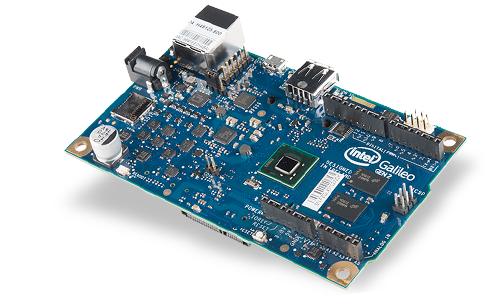
\includegraphics[width=200px,height=120px]{iot_galileo.png}
\end{figure}	

\end{frame}


\section{Struktur ToDo} 
\begin{frame}
\frametitle{ToDo}
\begin{itemize}
\item Idee und Zielsetzung (Stichworte sind vorhanden und muss noch in Sätze gefasst werden)
\item Unterkapitel Ziele für die Energieeinsparung 2050
\item Unterkapitel Strom-Landung und -Entladung innerhalb eines Transistors
\item Kapitel Resultate fertigstellen
\item Fazit mit Diskussion erstellen
\end{itemize}

\end{frame}

\begin{frame}
\frametitle{Resultate in Roh­form} 
\Huge Präsentation: Diagramme im Anhang
\end{frame}

\section{Struktur Resultate}
\begin{frame}
\frametitle{Resultate} 
\begin{minipage}{0.8\textwidth}

\begin{filecontents}{dataset}
Pos	Name	Bench1	Bench2	Bench3	time1	time2	time3	medbench	medtime	energymWh	power
1	nop	431.9	432	432	129147	129147	129147	432	129.147	98.565	2.74752
2	nop\_nop	430.2	430.4	430.3	145291	145291	145291	430.3	145.291	110.45	2.736708
3	nop\_nop\_nop	431.1	431.1	431.1	161435	161434	161434	431.1	161.434	122.95	2.741796
4	addl\_0	431.4	431.8	431.5	145292	145291	145291	431.5	145.291	110.758	2.74434
5	addl\_32	435.3	435.2	435.5	145291	145291	145291	435.3	145.291	111.733	2.768508
6	subl\_0	431.4	432.1	431.4	145291	145291	145292	431.6	145.291	110.783	2.744976
7	subl\_32	435	435.2	435.3	145291	145291	145291	435.2	145.291	111.707	2.767872
8	shr\_0	432.8	432.8	433.5	177578	177579	177579	432.9	177.579	135.811	2.753244
9	shr\_32	432.7	432.6	432.9	177578	177578	177578	432.7	177.578	135.747	2.751972
10	shl\_0	433.1	432.9	432.9	177579	177579	177579	432.9	177.579	135.811	2.753244
11	shl\_32	432.7	432.9	433.2	177578	177578	177578	432.9	177.578	135.81	2.753244
12	imull\_0	427.9	427.3	427.4	226008	226008	226008	427.4	226.008	170.653	2.718264
13	imull\_32	429.7	429.5	429.9	226008	226008	226008	429.7	226.008	171.571	2.732892
14	inc\_8	436.4	435.6	435.7	145292	145291	145291	435.9	145.291	111.887	2.772324
15	dec\_8	433.9	434.4	434.6	161434	161434	161434	434.4	161.434	123.891	2.762784
16	and\_0	434.7	435.2	435.1	145292	145291	145291	435	145.291	111.656	2.7666
17	and\_32	428.6	429.7	430.6	145291	145291	145292	429.7	145.291	110.296	2.732892
18	or\_0	436	435.3	434.9	145291	145291	145291	435.35	145.291	111.746	2.768826
19	or\_32	429.8	431.2	431.4	145291	145291	145291	431.1	145.291	110.655	2.741796
20	xor\_0	432.5	431.5	431.5	145291	145292	145292	431.6	145.292	110.784	2.744976
21	xor\_32	434.2	435	435	145291	145292	145291	434.7	145.291	111.579	2.764692
\end{filecontents}



\begin{figure}[h] 
    \centering
    \begin{tikzpicture} 
        \begin{axis}[
            ybar,
            scale only axis,
            xlabel= Benchmarks,
            width = 0.85\textwidth,
            height = 0.25\textheight,
            y axis line style=blau_2b!100!black,
            ylabel= Leistungsvbrauch in W,
            % height = 80mm,
            ymin = 2.688264,
            ymax = 2.801052,
            xmin = 0,
            xmax = 22,
            bar width = 2mm,
            axis x line* = bottom,
            axis y line* = left,
            xticklabel style={rotate=90},
            xticklabels from table = {dataset}{Name},
            xtick = {1,...,21},
            bar shift = -1mm,
            y tick label style = {/pgf/number format/use comma},
            legend style = {at={(0.5, 1.025)}, anchor = south east, legend columns = -1, draw=none, area legend},
            area legend,
            extra y ticks ={2.688264},
            extra y tick style = {grid=none, yticklabel style={yshift=2.5mm, xshift=1.9mm, rotate=0, inner sep=.5pt}},
            extra y tick labels = {
\includegraphics{almost_equals.eps}}
            ]
            \addplot+[mark=none, fill=blau_2a, draw = blau_2b] table[x=Pos, y=power, fill=red] {dataset};
            \legend{Leistungsverbrauch}
        \end{axis} 
        \begin{axis}[
            ybar,
            scale only axis,
            width = 0.85\textwidth,
            height = 0.25\textheight,
            y axis line style=gruen_4b!100!black,
            axis y line* = right,
            axis x line = none,
            ylabel = Durchlaufszeit in s,
            % height = 80mm,
            xmin = 0,
            xmax = 22,
            ymin = 0,
            xticklabel style={rotate=90},
            xticklabels from table = {dataset}{Name},
            xtick = {1,...,21},
            ymax = 246.008,
            ymin = 109.147,
            bar width = 2mm,
            bar shift = 1mm,
            legend style = {at={(0.5, 1.025)}, anchor = south west, legend columns = -1, draw=none, area legend},
            area legend,
            extra y ticks ={109.147},
            extra y tick style = {grid=none, yticklabel style={yshift=2.5mm, xshift=-1.6mm, rotate=0, inner sep=.5pt}},
            extra y tick labels = {
\includegraphics{almost_equals.eps}},
            ]
            \addplot+[mark=none,  fill=gruen_4a, draw = gruen_4b,] table[x=Pos, y=medtime] {dataset};
            \legend{Durchlaufszeit}
        \end{axis}
    \end{tikzpicture}
    \caption{Ausführung aller Benchmarks auf dem Galileo Board}
    \label{fig:benchmarks_galileo}
\end{figure}


\end{minipage}
\end{frame}





\end{document}

